%%%%%%%%%%%%%%%%%%%%%%%%%%%%%%%%%%%%%%%%%
% Beamer Presentation
% LaTeX Template
% Version 1.0 (10/11/12)
%
% This template has been downloaded from:
% http://www.LaTeXTemplates.com
%
% License:
% CC BY-NC-SA 3.0 (http://creativecommons.org/licenses/by-nc-sa/3.0/)
%
%%%%%%%%%%%%%%%%%%%%%%%%%%%%%%%%%%%%%%%%%

%----------------------------------------------------------------------------------------
%	PACKAGES AND THEMES
%----------------------------------------------------------------------------------------

\documentclass{beamer}

\mode<presentation> {

% The Beamer class comes with a number of default slide themes
% which change the colors and layouts of slides. Below this is a list
% of all the themes, uncomment each in turn to see what they look like.

%\usetheme{default}
%\usetheme{AnnArbor}
%\usetheme{Antibes}
%\usetheme{Bergen}
%\usetheme{Berkeley}
%\usetheme{Berlin}
%\usetheme{Boadilla}
%\usetheme{CambridgeUS}
%\usetheme{Copenhagen}
%\usetheme{Darmstadt}
%\usetheme{Dresden}
%\usetheme{Frankfurt}
%\usetheme{Goettingen}
%\usetheme{Hannover}
%\usetheme{Ilmenau}
%\usetheme{JuanLesPins}
%\usetheme{Luebeck}
\usetheme{Madrid}
%\usetheme{Malmoe}
%\usetheme{Marburg}
%\usetheme{Montpellier}
%\usetheme{PaloAlto}
%\usetheme{Pittsburgh}
%\usetheme{Rochester}
%\usetheme{Singapore}
%\usetheme{Szeged}
%\usetheme{Warsaw}

% As well as themes, the Beamer class has a number of color themes
% for any slide theme. Uncomment each of these in turn to see how it
% changes the colors of your current slide theme.

%\usecolortheme{albatross}
%\usecolortheme{beaver}
%\usecolortheme{beetle}
%\usecolortheme{crane}
%\usecolortheme{dolphin}
%\usecolortheme{dove}
%\usecolortheme{fly}
%\usecolortheme{lily}
%\usecolortheme{orchid}
%\usecolortheme{rose}
%\usecolortheme{seagull}
%\usecolortheme{seahorse}
%\usecolortheme{whale}
%\usecolortheme{wolverine}

\usefonttheme{serif} 

%\setbeamertemplate{footline} % To remove the footer line in all slides uncomment this line
%\setbeamertemplate{footline}[page number] % To replace the footer line in all slides with a simple slide count uncomment this line

\setbeamertemplate{navigation symbols}{} % To remove the navigation symbols from the bottom of all slides uncomment this line
}

\usepackage{graphicx} % Allows including images
\usepackage{booktabs} % Allows the use of \toprule, \midrule and \bottomrule in tables
\usepackage[T1]{fontenc}
\usepackage[utf8]{inputenc}
\usepackage{amsmath}
\usepackage{color}
\usepackage[czech]{babel}
\usepackage{lmodern}  
\usepackage{rotating}
\usepackage{scrextend}
\usepackage{pifont}
\usepackage{hyperref}
\usepackage{bm}

%----------------------------------------------------------------------------------------
%	TITLE PAGE
%----------------------------------------------------------------------------------------

\title[Týden 3]{Praktikum z ekonometrie - Týden 3} % The short title appears at the bottom of every slide, the full title is only on the title page

\author{VŠE Praha} % Your name
\institute[4EK417] % Your institution as it will appear on the bottom of every slide, may be shorthand to save space
{
% Your institution for the title page
\medskip
\textit{Tomáš Formánek} % Your email address
}
\date{} % Date, can be changed to a custom date

\begin{document}

\begin{frame}
\titlepage % Print the title page as the first slide
\end{frame}

\begin{frame}
\frametitle{Outline} % Table of contents slide, comment this block out to remove it
\tableofcontents % Throughout your presentation, if you choose to use \section{} and \subsection{} commands, these will automatically be printed on this slide as an overview of your presentation
\end{frame}

%----------------------------------------------------------------------------------------
%	PRESENTATION SLIDES
%---------------------------------------------------------------------------------------
\section{Variance vs. Bias} 


%------------------------------------------------


\begin{frame}
\frametitle{Some trade-offs in econometrics \& data analysis}

\begin{itemize}
  \item Prediction accuracy versus interpretability. 
  \\Linear models are easy to interpret; nonparametric classifiers are not.
  \vspace{0.2cm}
  \item Good fit versus over-fit or under-fit.
  \\ How do we know when the fit is just right?
  \vspace{0.2cm}
  \item Parsimony versus black-box.
  \\We often prefer a simpler model involving fewer variables over a black-box predictor involving them all.
\end{itemize}


\end{frame}


%------------------------------------------------



\begin{frame}
\frametitle{Variance vs. Bias}
% y = sin(x)+u
\begin{figure}
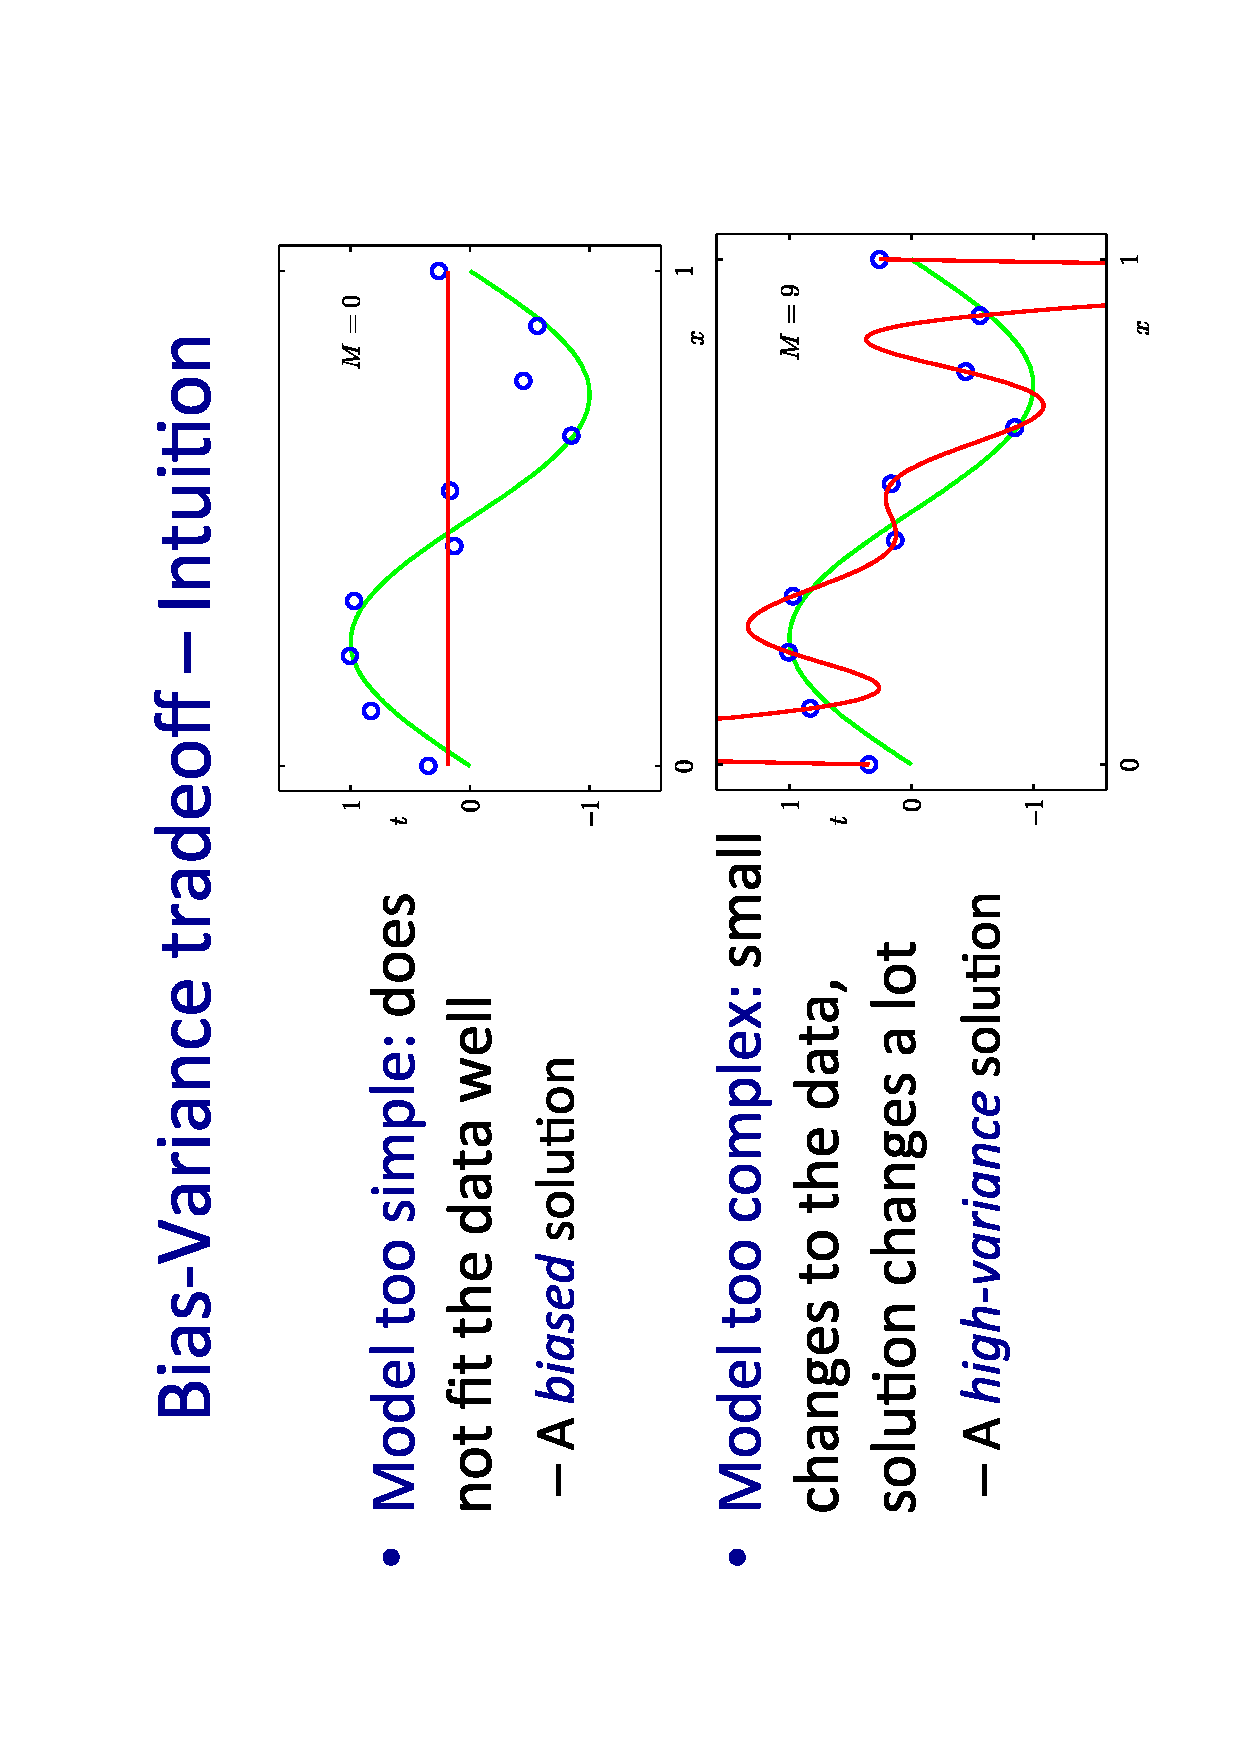
\includegraphics[angle=270,scale=0.35]{IMG/VarBias.pdf}
\end{figure}
\end{frame}



%------------------------------------------------


\begin{frame}
\frametitle{Variance vs. Bias}

Suppose we fit a model $\hat{\mathit{f}}(\bm{x})$ to some training data $\textnormal{Tr}=\left\lbrace y_i, \bm{x}_i \right\rbrace _1 ^n$ and we wish to see how well it performs.

\begin{itemize}
\item We could compute the average squared prediction error over $\textnormal{Tr}$:
$$ \textit{MSE}_{\textnormal{Tr}} = \frac{1}{n}
   \left[y_i - \hat{\mathit{f}}(\bm{x}_i) \right]^2 $$
\end{itemize}

When searching for the "best" model by minimizing $ \textit{MSE}$, the above statistic would lead to over-fit models.
\vspace{0.3cm}
\begin{itemize}
\item Instead, we should (if possible) compute the $ \textit{MSE}$ using fresh test
data $\textnormal{Te}=\left\lbrace y_i, \bm{x}_i \right\rbrace _1 ^m$:
$$ \textit{MSE}_{\textnormal{Te}} = \frac{1}{m}
   \left[y_i - \hat{\mathit{f}}(\bm{x}_i) \right]^2 $$
\end{itemize}


\end{frame}

%------------------------------------------------
\begin{frame}
\frametitle{Variance vs. Bias}

Suppose we have a model $\hat{\mathit{f}}(\bm{x})$, fitted to some training data $\textnormal{Tr}$ and let $\left\lbrace y_0, \bm{x}_0 \right\rbrace$ be a test observation drawn from the population. \\If the true model is 
$y_i = \mathit{f}(\bm{x}_i) + \varepsilon_i$, [with $\mathit{f}(\bm{x}_i)= \textnormal{E}(y_i | \bm{x}_i $)],\\
then the \textit{expected test MSE} is

$$ \textnormal{E}(\textit{MSE}_0)
   =\textnormal{E}[y_0- \hat{\mathit{f}}(\bm{x}_0)]^2 
   = Var(\hat{\mathit{f}}(\bm{x}_0))
   + [Bias(\hat{\mathit{f}}(\bm{x}_0))]^2
   + Var(\varepsilon_0), $$

where $Bias(\hat{\mathit{f}}(\bm{x}_0)) 
       = \textnormal{E}[\hat{\mathit{f}}(\bm{x}_0)]
       - \mathit{f}(\bm{x}_0)$,
\\ \hspace{1cm} $\varepsilon_0$ is the irreducible error: $\textnormal{E}(\textit{MSE}_0)$ can never lie below it,
\\ \hspace{1cm} all three RHS elements are non-negative,
\vspace{0.5cm} 
\\The above equation refers to the average test $\textit{MSE}$ that we would obtain if we repeatedly estimated $\mathit{f}(\bm{x})$ using a large number of training sets and then tested each $\hat{\mathit{f}}(\bm{x})$ at $\bm{x}_0$.


\end{frame}
%------------------------------------------------



\begin{frame}
\frametitle{Variance vs. Bias}

$$ \textnormal{E}(\textit{MSE}_0)
   =\textnormal{E}[y_0- \hat{\mathit{f}}(\bm{x}_0)]^2 
   = Var(\hat{\mathit{f}}(\bm{x}_0))
   + [Bias(\hat{\mathit{f}}(\bm{x}_0))]^2
   + Var(\varepsilon_0), $$

\vspace{0.5cm} 

As the flexibility (complexity) of ${\mathit{f}}(\bm{x})$ increases, 
\\the variance of $\hat{\mathit{f}}(\bm{x})$ increases and its bias decreases.
\vspace{0.5cm} 
\\Choosing the flexibility (complexity and -generally speaking- specification) of the model based on average test errors amounts to \\ 
\textbf{Variance vs. Bias} trade-off.



\end{frame}


%------------------------------------------------



\begin{frame}
\frametitle{Variance vs. Bias}

\begin{center}
Variance vs. Bias: three sample datasets.
\end{center}

\begin{figure}
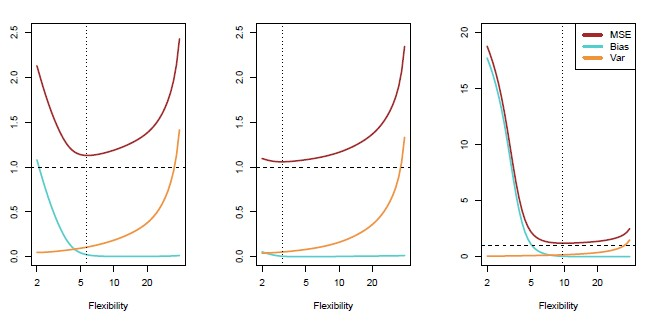
\includegraphics[scale=0.5]{IMG/VarBias_ex_2.jpg}
\end{figure}

\end{frame}





%------------------------------------------------
\section{$k$-Fold Cross Validation} 

%------------------------------------------------

\begin{frame}
\frametitle{$k$-Fold Cross Validation}

Test error vs. training error concept:
\begin{itemize}
\item The test error is the average error that results from using a statistical learning method to predict the response on a new observation (not used for training).
\item Training error can be easily calculated by applying the statistical learning method to the observations used in its training.
\item Training error is not a good approximation for test error (out-of sample predictive properties of the model).
\item Usually, training error dramatically underestimates test error.
\end{itemize}
\bigskip
Cross-validation is based on re-sampling (similar to bootstrap).\\
\medskip
Repeatedly fit a model of interest to samples formed from the training set \& make ``test sample'' predictions, in order to obtain additional information about predictive properties of the model.\\

\end{frame}

%------------------------------------------------

\begin{frame}
\frametitle{$k$-Fold Cross Validation}
Cross-validation is based on re-sampling (similar to bootstrap).\\
\medskip
Repeatedly fit a model of interest to samples formed from the training set \& make ``test sample'' predictions, in order to obtain additional information about predictive properties of the model.\\
~\\
$k$-Fold Cross Validation example for $k=3$:

\begin{figure}
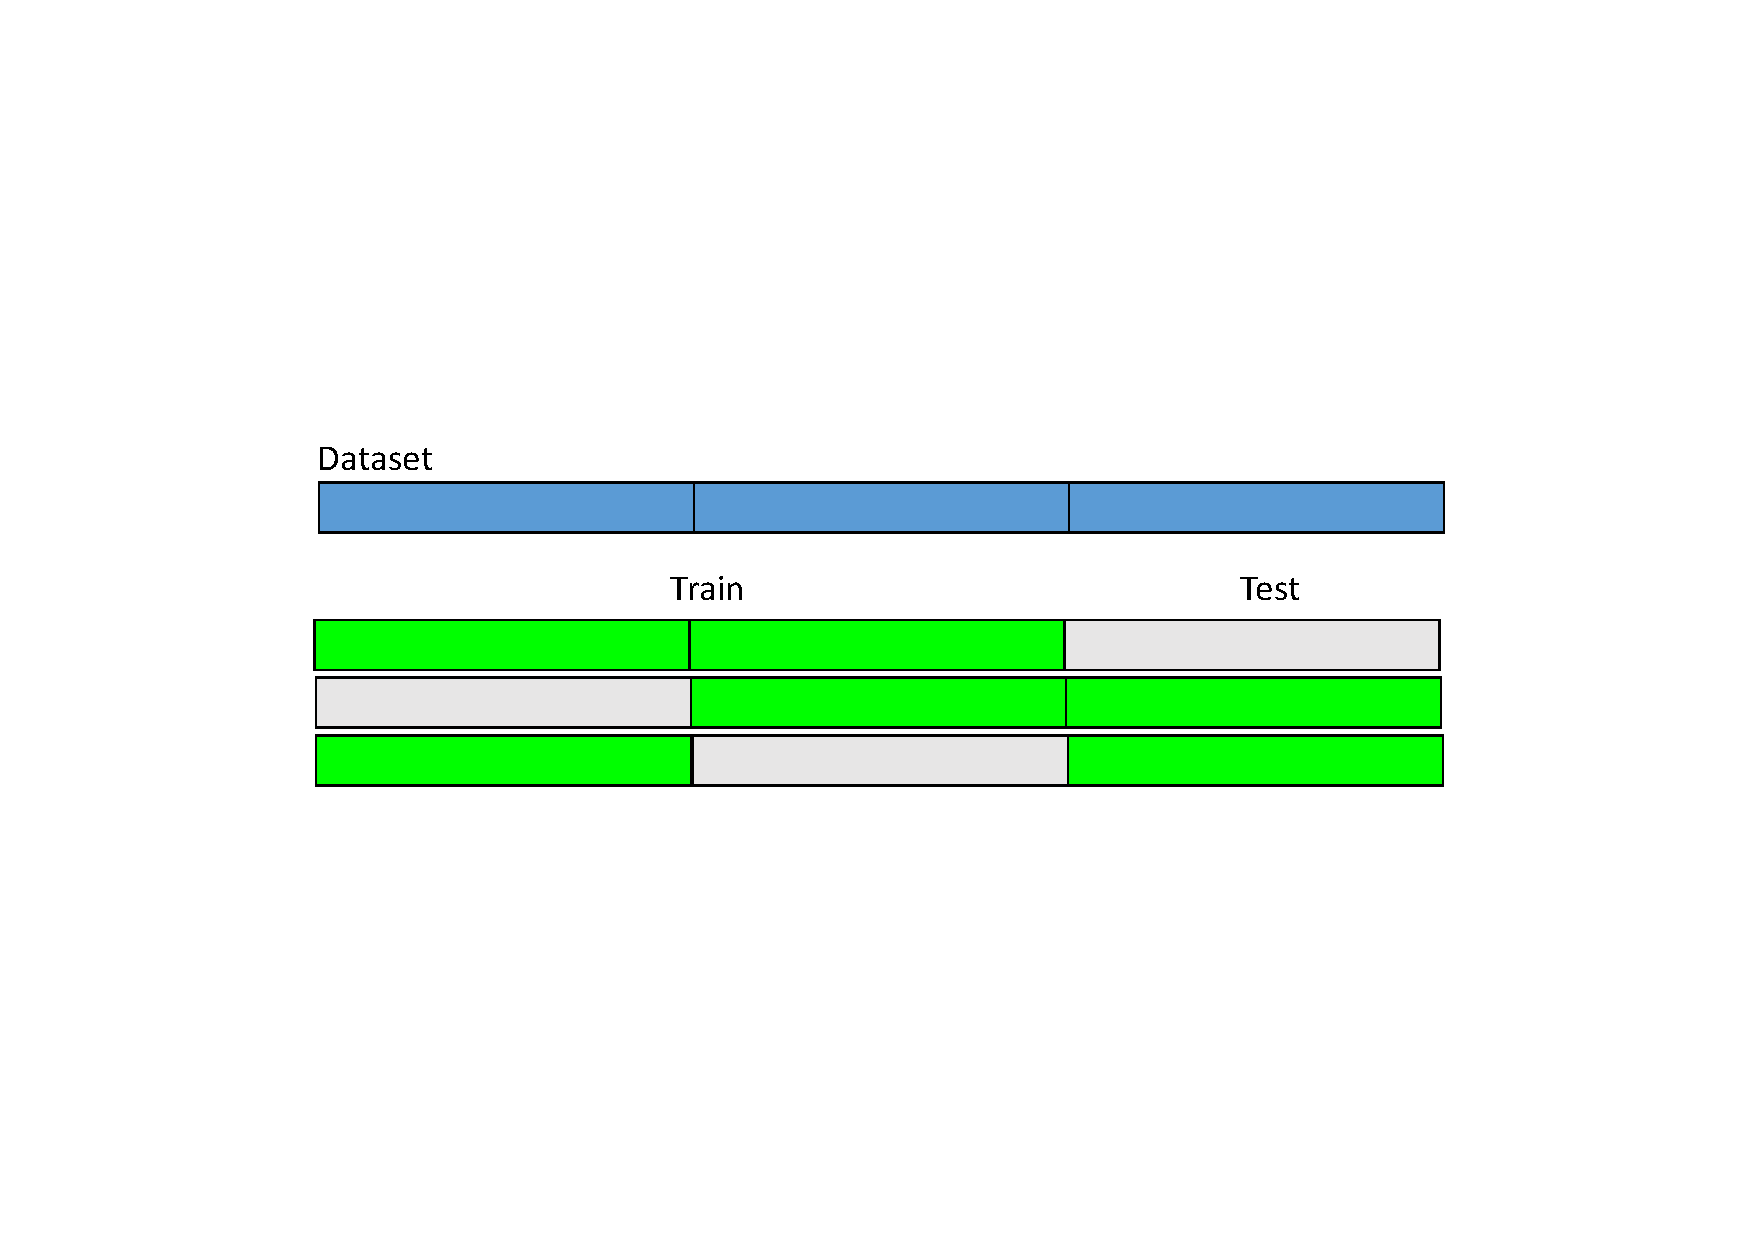
\includegraphics[trim=100 200 100 200,clip,width=7cm]{IMG/kFCV.pdf}
\end{figure}

\end{frame}


%------------------------------------------------

\begin{frame}
\frametitle{$k$-Fold Cross Validation}

\begin{itemize}
  \item In $k$-Fold Cross-Validation ($k$FCV), the original sample is randomly partitioned into $k$ roughly equal subsamples (divisibility). 
  \item Of the $k$ subsamples, a single subsample is retained as the validation data for testing the model, and the remaining $(k-1)$ subsamples are used as training data. 
  \item The cross-validation process is then repeated $k$ times (the $k$ folds), with each of the $k$ subsamples used exactly once as the validation data. 
  \item The $k$ results from the folds can then be averaged to produce a single estimation. 
  \item $k = 5$ or $k=10$ is commonly used, yet $k$ remains an unfixed parameter.
\end{itemize}  

\end{frame}


%------------------------------------------------


\begin{frame}
\frametitle{$k$-Fold Cross Validation}

\begin{center}
$k$FCV example for $k=5$: \\
(random sampling, no replacement)
\begin{figure}
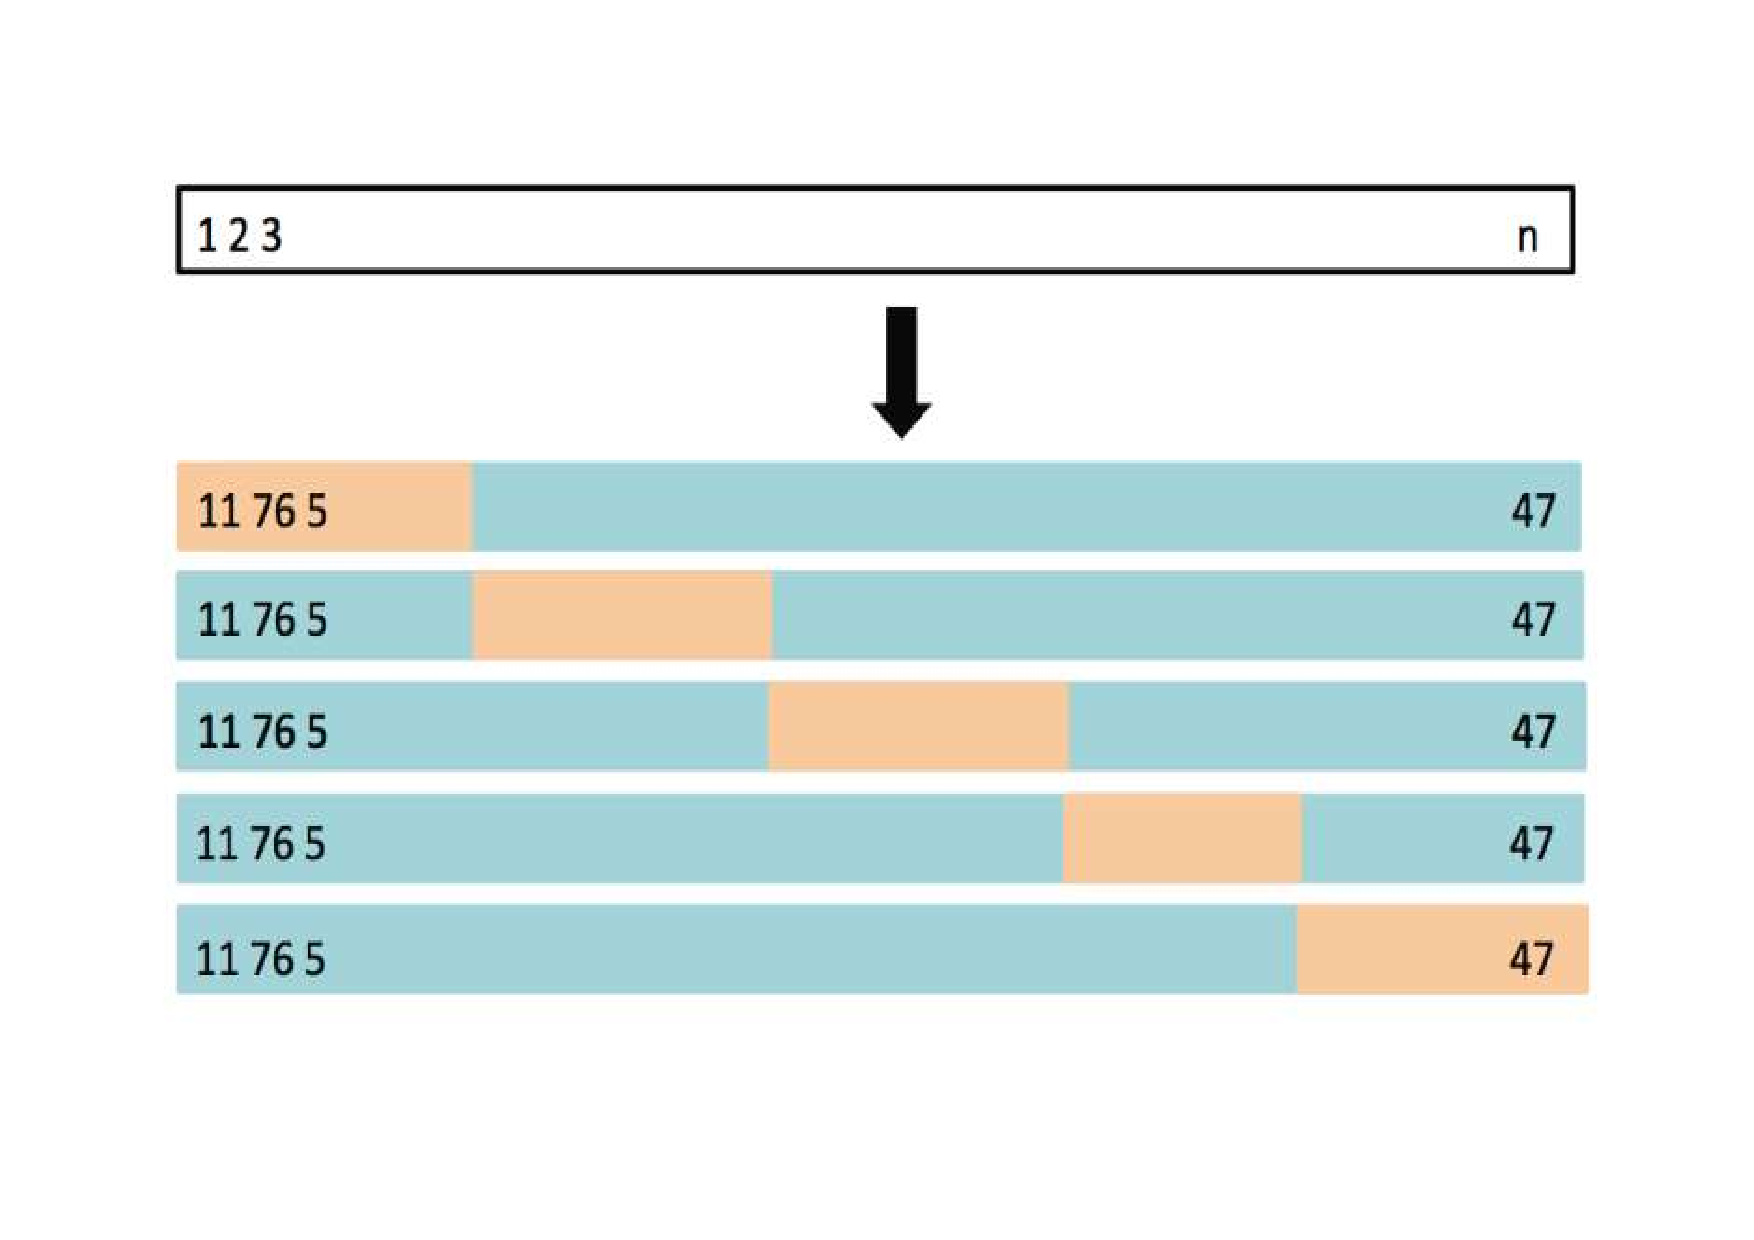
\includegraphics[width=0.6\linewidth]{IMG/kFCV2.pdf}
\end{figure}
\end{center}

\end{frame}


%------------------------------------------------


\begin{frame}
\frametitle{$k$-Fold Cross Validation algorithm recap}

\begin{enumerate}
  \item We randomly divide the data set of into $k$ folds ($k = 5$ or 10).
  \vspace{0.2cm}
  \item The first fold is treated as a validation set, and the method is fit on the remaining $(k-1)$ folds. The $\textit{MSE}$ is computed on the observations in the held-out fold. The process is repeated $k$ times, taking out a different part each time.
   \vspace{0.2cm}
  \item By averaging the $k$  $\textit{MSE}$  estimates $\left\lbrace \textit{MSE}_1 , \dots, \textit{MSE}_k \right\rbrace$, we get an estimated validation (test) error rate for new observations: $\textit{CV}_{(k)}$.
\end{enumerate}
\vspace{0.5cm}
In a bootstrap-like approach (yet, no replacement in individual samples), we may repeat steps 1 to 3 multiple times (say, $R=500$). This renders a more precise $\textit{CV}_{(k)}$ estimate and its expected distribution.

\end{frame}

%------------------------------------------------


\begin{frame}
\frametitle{$k$-Fold Cross Validation statistics}


$ \textit{CV}_{(k)}= \frac{1}{k}\displaystyle\sum_{s=1}^{k} \textit{MSE}_s $
\vspace{0.3cm}

\begin{labeling}{where}
\item [where] $\textit{CV}_{(k)}$ is the $k$-fold \textit{CV} estimate,
\item [ ] $k$ is the number of $k$FC folds generated (say, 5 or 10),
\item [ ] $\textit{MSE}_s = \frac{1}{m_s} \sum_{i \in C_s}^{}(y_i - \widehat{y}_i)^2 $ \\ where $m_s$ and $C_s$ refer to ``test sample'' observations for each of the $k$ train sample - test sample steps.
\end{labeling}
\vspace{0.3cm}

Usually, we repeat the train sample - test sample cast repeatedly.\\ Say, for $R=500 \Rightarrow$ 500 $\textit{CV}_{(k)}$ statistics are estimated and averaged into a final Cross-validated $\textit{MSE}$ statistics
\vspace{0.3cm}

As we compare predictions from two or more models, 
\\we look for the lowest $\textit{CV}_{(k)}$. 


\end{frame}




%------------------------------------------------

\begin{frame}

\frametitle{$k$FCV - final remarks}

\begin{enumerate}

  \item We tend to use $k$FCV with $k = 5$ or $k = 10$, as these values have been shown empirically to yield test error rate estimates that suffer neither from excessively high bias nor from very high variance
  \vspace{0.5cm}
  \item The advantage of $k$FCV over repeated random sub-sampling is that all observations are used for both training and validation, and each observation is used for validation exactly once.
  
\end{enumerate}  

\end{frame}

%------------------------------------------------
\section{Walk-forward testing} 
%------------------------------------------------

%------------------------------------------------

\begin{frame}
\frametitle{Walk-forward testing}

Walk forward test is a model-evaluation technique in which we optimize the parameter values on a past segment of (market) data (``in-sample''), then verify the performance of the system by testing it forward in time on data following the optimization segment (``out-of-sample''). \\
(remember Chow test 1 vs. Chow test 2)
\medskip
We evaluate the system based on how well it performs on the test data (``out-of-sample''), not the data it was optimized on.
\medskip
The process can be repeated over subsequent time segments. 
\medskip
The following illustration shows how the process works.
\end{frame}

%------------------------------------------------


\begin{frame}
\frametitle{Walk-forward testing}

\begin{center}
\begin{figure}
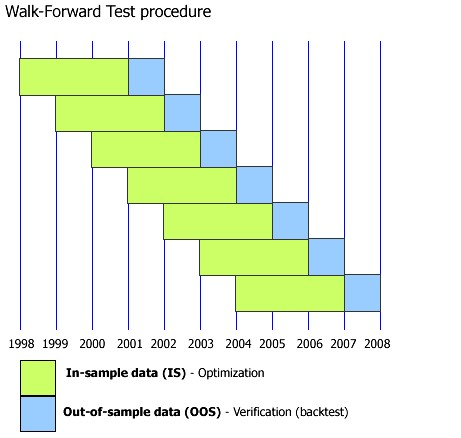
\includegraphics[width=0.6\linewidth]{IMG/walkfwd2.jpg}
\end{figure}
\end{center}

\end{frame}

%------------------------------------------------

\begin{frame}
\frametitle{Walk-forward testing}

\begin{itemize}
\item The premise of performing several optimization/tests steps over time is that the recent past is a better foundation for selecting system parameter values than the distant past. 
\bigskip
\item Usual assumptions/setup:
\medskip
\begin{itemize}
\item Out-of-sample segment immediately follows in-sample segment
\medskip
\item The length of out-of-sample segment equals to the walk-forward step
\end{itemize}
\end{itemize}

\end{frame}

%------------------------------------------------

\begin{frame}
\frametitle{Missing data?}
\begin{figure}

\includegraphics[width=0.15\linewidth]{IMG/Complex_topic.pdf}
\end{figure}

\begin{center}
Missing data! 
\end{center}

\end{frame}

%------------------------------------------------

%----------------------------------------------------------------------------------------
\section{Missing data \& multiple imputation}
%------------------------------------------------

\begin{frame}
\frametitle{Missing data}


\begin{itemize}
  \item The nature of missing data
  \item Traditional treatment of missing data
  \item Modern approaches to missing data
  \item Missing dependent variable data

\end{itemize}


\end{frame}

%------------------------------------------------

\begin{frame}
\frametitle{The nature of missing data}

\begin{itemize}
  \item[] Missing completely at random (\textit{MCAR})
  \begin{itemize}
  \item The probability that an observation $X_i$ is missing is unrelated to the value of $X_i$ or to the value of any other variables.
  \item Any piece of data is equally likely to be missing.
  \item Analyses based on data with \textit{MCAR} observations remain unbiased. We may lose power (increased standard errors), but the estimated parameters are not biased by the absence of data.
  \end{itemize}
  \vspace{0.2cm}
  \item[] Missing at random (\textit{MAR})
  \begin{itemize}
  \item Data meets the requirement that missingness does not depend on the value of $X_i$ after controlling for another variable in our analysis.
  \item For example, data are MCAR in a specific (demographic) subgroup. 
  \end{itemize}
  \vspace{0.2cm}
  \item[] Missing Not at Random (\textit{MNAR})
  \begin{itemize}
  \item Missigness of $X_i$ depends on its value (e.g. income in surveys)
  \item The only way to obtain an unbiased estimates of (regression) parameters is to model the missingness.
  \end{itemize}
\end{itemize}


\end{frame}

%------------------------------------------------

\begin{frame}[fragile] % Need to use the fragile option when verbatim is used in the slide
\frametitle{Traditional treatment of missing data}


\textbf{Listwise deletion (complete cases analysis)}
\vspace{0.2cm}
  \begin{itemize}
  \item  We omit all rows with missing data – missing information for at least one variable in the $i$-th individual observation. Then, we run our analyses on the observations that remain. This often results in a substantial decrease in sample size. Under the assumption that data are missing completely at random, LRMs lead to unbiased parameter estimates – still, we lose power due to exclusion of (potentially large number of) observations.
  \end{itemize} 

\begin{block}{R code}
\begin{verbatim}
newData <- data[complete.cases(data)==T, ] 
# data is a data.frame
# or
newData <- na.omit(data) 
\end{verbatim}
\end{block}

\end{frame}

%------------------------------------------------

\begin{frame}
\frametitle{Traditional treatment of missing data}


\textbf{Hot deck imputation}
\vspace{0.2cm}
  \begin{itemize}
  \item  Historically used by the US Census Bureau (since 1950’s). Respondent’s missing data were replaced by observed replacement data – drawn at random from a group of similar participants. Suitable, given only a few missing observations need to be replaced and given the draw is random.
  \end{itemize} 

\end{frame}


%------------------------------------------------


\begin{frame}
\frametitle{Traditional treatment of missing data}


\textbf{Mean substitution}
\vspace{0.2cm}
  \begin{itemize}
  \item[\ding{51}] Simple
  \item[\ding{55}] In simple linear regression models (SLRMs), this adds no new information but increases sample size – that leads to underestimated standard errors only.
  \end{itemize} 
  \vspace{0.2cm}
\textbf{Example:} Data on salary and citation level of publications. 62 cases with complete data and 7 cases for which the citation index was missing. Correlations and regression coefficients were compared as follows:

\begin{table}
\begin{tabular}{l c c c c}
\toprule
Analysis & $n$ & $corr$ & $\widehat{\beta}_1$ & $\textit{s.e.}(\widehat{\beta}_1)$\\
\midrule
Complete cases only & 62 & .55 &  310.747 & 60.95 \\
With mean substitution & 69 & .54 &  310.747 & 59.12 \\
\bottomrule
\end{tabular}

\end{table}

\end{frame}

%------------------------------------------------

\begin{frame}
\frametitle{Traditional treatment of missing data}

\textbf{Regression substitution}
  \begin{itemize}
  \item Uses linear regression (auxiliary LRM) to predict what the missing values of regressors should be, on the basis of other variables that are present.
  \item For SLRMs, the same problem of error variance as in mean substitution remains. We do not add more information but we increase the sample size and (spuriously) reduce the standard error.
  \item May be useful for MLRMs.
   \end{itemize}
  \vspace{0.2cm}
\textbf{Stochastic regression substitution}
  \begin{itemize}
  \item This approach adds a randomly sampled residual term from the normal (or other) distribution to each value estimated by regression substitution. Adding a bit of random error to each substitution reduces, but does not eliminate, the problem of spurious reduction of the standard errors.
   \end{itemize}

\end{frame}


%------------------------------------------------

\begin{frame}
\frametitle{Modern Approaches to missing data}

\textbf{Maximum Likelihood Expectation-Maximization}
  \begin{itemize}
  \item Computationally complex, maximum likelihood approach to the estimation of missing values Many approaches exist (e.g. the Expectation-Maximization algorithm)
  \item[] \scriptsize{\url{https://www.uvm.edu/~dhowell/StatPages/Missing_Data/Missing-Part-Two.html}}
   \end{itemize}
 
\end{frame}

%------------------------------------------------



\begin{frame}
\frametitle{Modern Approaches to missing data}

\textbf{Multiple Imputation (MI) }
  \begin{itemize}
  \item[] R: $\left\lbrace \textnormal{mice}  \right\rbrace , \,\, \left\lbrace \textnormal{mi}  \right\rbrace, \,\, \left\lbrace \textnormal{Amelia}  \right\rbrace, \, $ \dots
  \vspace{0.5cm}
  \item[] MI motivation and algorithm
  \vspace{0.2cm}
  \begin{itemize}
  \item Create several (say, 5) “imputed” values for each missing value $X_{ij}$. Each of the (5) versions of imputed data values are estimated/predicted using a separate ML approach from the data frame observed (different “model” is used for each imputation).
  \vspace{0.2cm}
  \item For SLRMs, this may be simplified into mean substitution augmented by adding random errors which reflect sampling variability of $X_j$.
  \end{itemize}
 \end{itemize}
 
\end{frame}


%------------------------------------------------


\begin{frame}
\frametitle{Modern Approaches to missing data}
\vspace{0.2cm}
\textbf{Multiple Imputation (contnd.) }
\vspace{0.2cm}
  \begin{itemize}
  \item[] How do we analyze estimates on data with MI?
  \begin{enumerate}
  \vspace{0.5cm}
  \item We use each set of imputed values to form a separate completed dataset (e.g., we get 5 datasets).
  \vspace{0.2cm}
  \item For each completed dataset, a standard analysis (LRM) can be run.
  \vspace{0.2cm}
  \item Inferences can be combined across MI-based datasets.
  \end{enumerate}
 \end{itemize}
 
\end{frame}

%------------------------------------------------


\begin{frame}

\frametitle{Modern Approaches to missing data}
\textbf{Multiple Imputation (contnd.) }
\begin{figure}
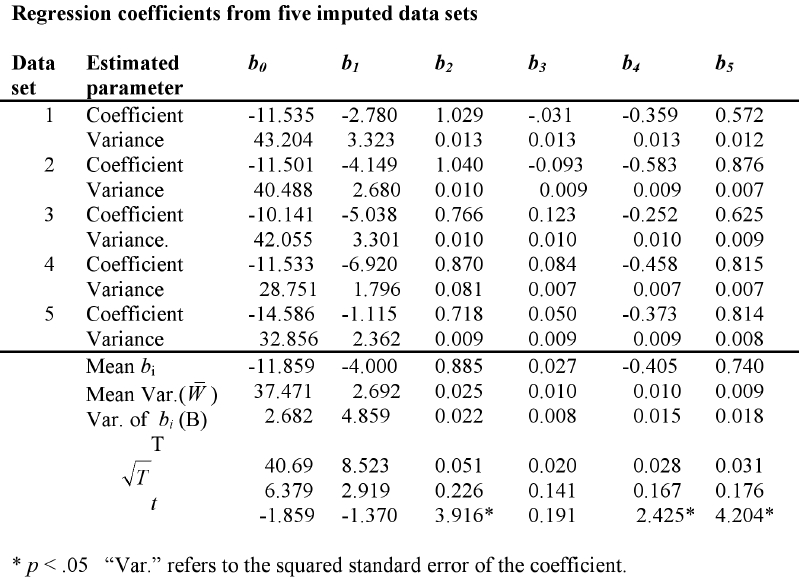
\includegraphics[width=0.7\linewidth]{IMG/mitable.jpg}
\end{figure}

\scriptsize{\url{https://www.uvm.edu/~dhowell/StatPages/Missing_Data/Missing-Part-Two.html}}

\end{frame}


%------------------------------------------------


\begin{frame}
\frametitle{Missing dependent variable data}

\textbf{Special considerations apply to missing dependent variable data}

\begin{itemize}
  \item If we can assume that data are missing completely at random \textit{(MCAR)}, we will lose power because of smaller sample sizes, but we will not have problems with biased estimates.
  \item If data are missing not at random \textit{(MNAR)}, the \textbf{only way to obtain an unbiased estimate of parameters is to model missingness}. In other words we need to use a model that accounts for the missing data.
  \item Broadly speaking, such models are:
  \begin{itemize}
    \item Censored Regression Models (e.g. duration analysis) 
    \item Truncated Regression Models 
    \item Sample Selection Correction models (Heckit)
    \item \dots
  \end{itemize}
\end{itemize}

\end{frame}


%------------------------------------------------



























%---------------------------------------------------------------------

\end{document}